\documentclass[paper=a4,fontsize=11pt]{article}
\usepackage{amsmath,amssymb,amsthm}
\usepackage[protrusion=true,expansion=true]{microtype}	
\usepackage{algorithm}
\usepackage{algpseudocode}
\usepackage[margin=1.5in]{geometry}
\usepackage{graphicx}
\setlength{\textfloatsep}{0.1cm}
\setlength{\floatsep}{0.1cm}
\begin{document}
\title{TCSS 343 - Assignment 3}
\author{Jake McKenzie}
\maketitle
In this problem use the Master Theorem to find and prove tight bounds for these recurrences (6 points each).\\\\
To solve this problem I used the master theorem taken from CLRS. I used a bit of a stronger statement than what was stated in the theorem but they are equivalent mathematically due to the nature of limits. I will include the theorem for the reader's benefit. To check my work I decided to include what I obtained using the Akra-Bazzi method.\\
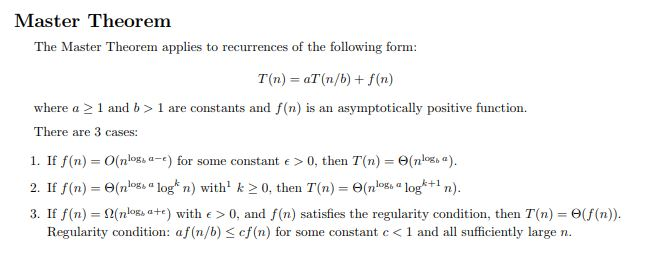
\includegraphics[width=\linewidth]{mastertheorem.JPG}
\begin{enumerate}
\item
\[
T(n) = \left\{
\begin{array}{cl}
c & \textrm{ if } n < 8\\
16T(n/8) + n\log{n} & \textrm{ if } n \geq 8
\end{array}
\right.
\]
\begin{align*}
\lim_{n\to\infty}{\frac{n\log{n}}{n^{\log_{8}{16}+\varepsilon}}}&=\lim_{n\to\infty}{\frac{n\log{n}}{n^{\frac{4}{3}+\frac{2}{3}}}}\\
&=\lim_{n\to\infty}{(\frac{n}{n})(\frac{\log{n}}{n})}\rightarrow0\\
T(n)&\in\Theta(n^{\frac{4}{3}})
\end{align*}
By Akra-Bazzi I obtain:\\
\begin{align*}
16(1/8)^{p}&=1\\
p&=\frac{4}{3}
\end{align*}
\begin{align*}
T(n) &\in \Theta(n^{p}(1+\int_{1}^{n}{\frac{u\log{u}}{u^{p+1}}du}))\\
&\in \Theta(-9n+10n^{\frac{4}{3}}-3n\log{n})\\
&\in \Theta(n^{\frac{4}{3}})\\
\end{align*}
\item
\[
T(n) = \left\{
\begin{array}{cl}
c & \textrm{ if } n < 4\\
8T(n/4) + n\log n & \textrm{ if } n \geq 4
\end{array}
\right.
\]
By Master Method I obtain:
\begin{align*}
    \lim_{n\to\infty}{\frac{n^{\frac{1}{3}}}{n^{\log_{8}{2}+\varepsilon}}}&=\lim_{n\to\infty}{\frac{n^{\frac{1}{3}}}{n^{\frac{1}{3}}}}\\
    &=\lim_{n\to\infty}{1}\rightarrow1\\
    &\in \Theta(n^{\frac{1}{3}}\log{n})\\
\end{align*}
By Akra-Bazzi I obtain:
\begin{align*}
    2(1/8)^{p}&=1\\
    p&=\frac{1}{3}
\end{align*}
\begin{align*}
    T(n) &\in \Theta(n^{p}(1+\int_{1}^{n}{\frac{u^{\frac{1}{3}}}{u^{p+1}}du}))\\
    &\in \Theta(n^{\frac{1}{3}}+n^{\frac{1}{3}}\log{n})\\
    &\in \Theta(n^{\frac{1}{3}}\log{n})\\
    \end{align*}
\end{enumerate}
\end{document}